\chapter{Experimental Results}\label{app:extra_experiments}

\section{Additive vs. Multiplicative Transforms for \(K=R=2\)}

\begin{table}[H]
\begin{center}
    \begin{tabular}{@{}lllllll@{}}
    \toprule
     \(n_s\) & \multicolumn{3}{l}{Additive} & \multicolumn{3}{l}{Multiplicative} \\ \midrule
        & \(\bar{M}(G)\) \% & (-)\% & (+)\% & \(\bar{M}(G)\) \% & (-)\% & (+)\%  \\ \midrule
        10 &\(4.76\) & \(4.46\) & \(5.05\) & \(4.64\) & \(4.32\) & \(4.96\) \\ 
        20 &\(3.55\) & \(3.33\) & \(3.77\) & \(3.36\) & \(3.15\) & \(3.58\) \\ 
        50 &\(2.23\) & \(2.09\) & \(2.37\) & \(2.24\) & \(2.09\) & \(2.38\) \\ 
        100 &\(1.52\) & \(1.43\) & \(1.6\) & \(1.5\) & \(1.41\) & \(1.59\) \\ 
        200 &\(1.06\) & \(0.991\) & \(1.12\) & \(1.07\) & \(1.01\) & \(1.14\) \\ 
        500 &\(0.646\) & \(0.608\) & \(0.684\) & \(0.681\) & \(0.637\) & \(0.725\) \\ 
        1000 &\(0.486\) & \(0.456\) & \(0.516\) & \(0.476\) & \(0.445\) & \(0.506\) \\ 
        2000 &\(0.335\) & \(0.315\) & \(0.356\) & \(0.336\) & \(0.316\) & \(0.357\) \\ 
        5000 &\(0.208\) & \(0.195\) & \(0.22\) & \(0.206\) & \(0.193\) & \(0.218\) \\ 
        10000 &\(0.14\) & \(0.132\) & \(0.149\) & \(0.15\) & \(0.141\) & \(0.16\) \\   \bottomrule
    \end{tabular}
\end{center}
\caption{Normalizing constant MAPE \(M(G)\) and and 95\(\%\) confidence intervals for \(K=R=2\)}
\label{tab:NC_MAPE_transforms_KR2}
\end{table}

\newpage

\begin{figure}[H]
\begin{center}
    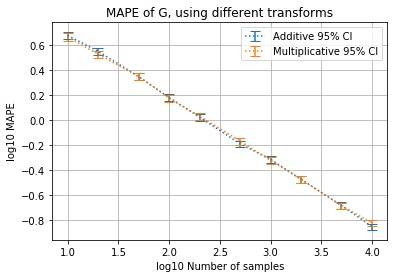
\includegraphics[width=0.6\textwidth]{figures/convergence_KR2.png}
\caption{Convergence plots of standard error and 95\% confidence intervals for the MAPE for different transforms. \(K=R=2\)}
\label{fig:Convergence_Transforms_KR2}
\end{center}
\end{figure}

\begin{figure}[H]
\begin{center}
\begin{subfigure}
    \centering
    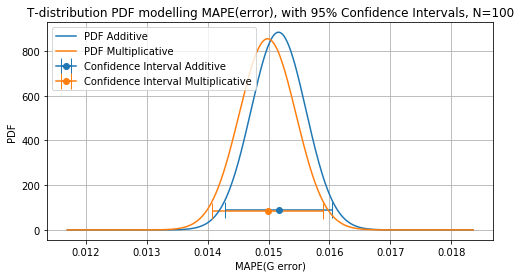
\includegraphics[width=0.5\textwidth]{figures/KR2N100_post.png}
\end{subfigure}
\begin{subfigure}
    \centering
    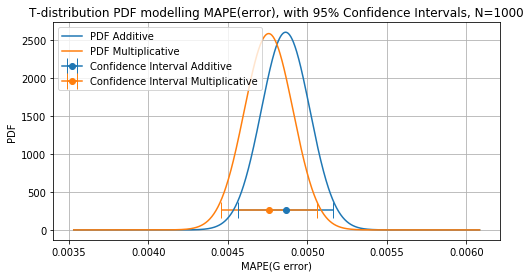
\includegraphics[width=0.5\textwidth]{figures/KR2N1000_post.png}
\end{subfigure}
\begin{subfigure}
    \centering
    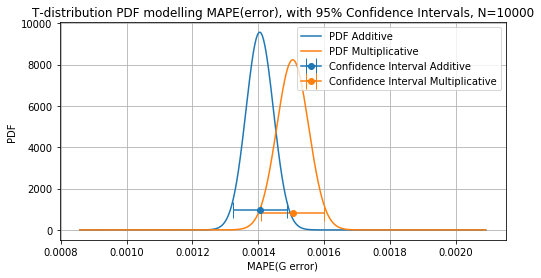
\includegraphics[width=0.5\textwidth]{figures/KR2N10000_post.png}
\end{subfigure}
\caption{ T - distributions of the true MAPE, given the estimated MAPE \(\bar{M}\) for different transforms. \(K=R=2\)}
\label{fig:Posterior_sigma_transforms_KR2}
\end{center}
\end{figure}

\newpage

\section{Additive vs. Multiplicative Transforms for \(K=R=4\)}

\begin{table}[H]
\begin{center}
    \begin{tabular}{@{}lllllll@{}}
    \toprule
     \(n_s\) & \multicolumn{3}{l}{Additive} & \multicolumn{3}{l}{Multiplicative} \\ \midrule
        & \(\bar{M}(G)\) \% & (-)\% & (+)\% & \(\bar{M}(G)\) \% & (-)\% & (+)\%  \\ \midrule
        10 &\(15.6\) & \(14.8\) & \(16.5\) & \(14.2\) & \(13.5\) & \(15\)  \\ 
        20 &\(11.9\) & \(11.2\) & \(12.5\) & \(10.2\) & \(9.62\) & \(10.7\)  \\ 
        50 &\(7.41\) & \(7.02\) & \(7.8\) & \(6.8\) & \(6.45\) & \(7.15\)  \\ 
        100 &\(5.2\) & \(4.95\) & \(5.45\) & \(4.71\) & \(4.47\) & \(4.94\)  \\ 
        200 &\(3.75\) & \(3.56\) & \(3.93\) & \(3.15\) & \(2.99\) & \(3.31\)  \\ 
        500 &\(2.32\) & \(2.2\) & \(2.44\) & \(2.08\) & \(1.98\) & \(2.18\)  \\ 
        1000 &\(1.66\) & \(1.58\) & \(1.74\) & \(1.5\) & \(1.42\) & \(1.58\)  \\ 
        2000 &\(1.22\) & \(1.15\) & \(1.28\) & \(1.03\) & \(0.976\) & \(1.08\)  \\ 
        5000 &\(0.734\) & \(0.696\) & \(0.772\) & \(0.641\) & \(0.609\) & \(0.672\)  \\ 
        10000 &\(0.518\) & \(0.492\) & \(0.544\) & \(0.478\) & \(0.453\) & \(0.502\)  \\   \bottomrule
    \end{tabular}
\end{center}
\caption{Normalizing constant MAPE \(M(G)\) and and 95\(\%\) confidence intervals for \(K=R=4\)}
\label{tab:NC_MAPE_transforms_KR4}
\end{table}


\begin{figure}[H]
\begin{center}
    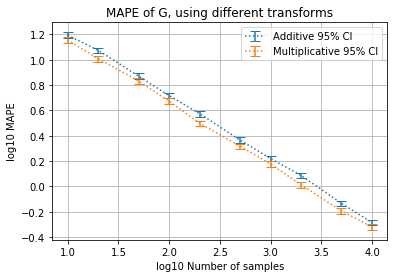
\includegraphics[width=0.6\textwidth]{figures/convergence_KR4.png}
\caption{Convergence plots of standard error and 95\% confidence intervals for the MAPE for different transforms. \(K=R=4\)}
\label{fig:Convergence_Transforms_KR4}
\end{center}
\end{figure}

\newpage

\begin{figure}[H]
\begin{center}
\begin{subfigure}
    \centering
    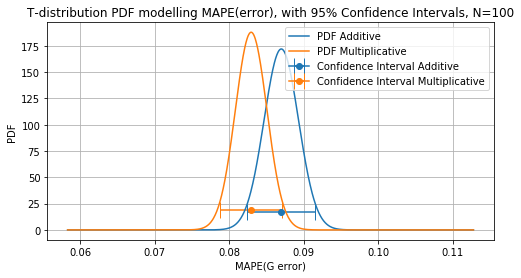
\includegraphics[width=0.5\textwidth]{figures/KR4N100_post.png}
\end{subfigure}
\begin{subfigure}
    \centering
    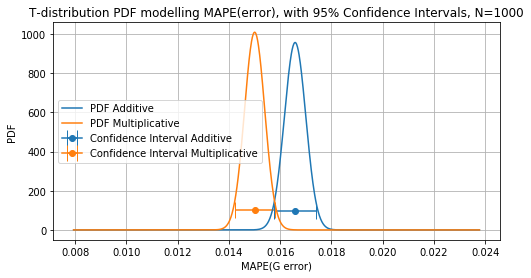
\includegraphics[width=0.5\textwidth]{figures/KR4N1000_post.png}
\end{subfigure}
\begin{subfigure}
    \centering
    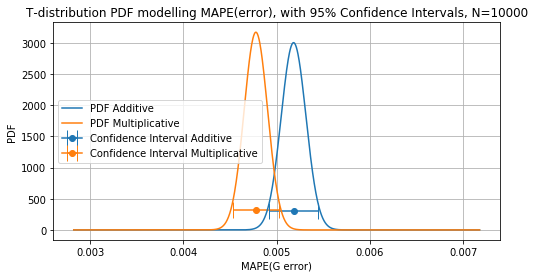
\includegraphics[width=0.5\textwidth]{figures/KR4N10000_post.png}
\end{subfigure}
\caption{ T - distributions of the true MAPE, given the estimated MAPE \(\bar{M}\) for different transforms. \(K=R=4\)}
\label{fig:Posterior_sigma_transforms_KR4}
\end{center}
\end{figure}

\newpage

\chapter{Usage Guide}
\section{Short guide for developers}

\begin{figure}[H]
\centering
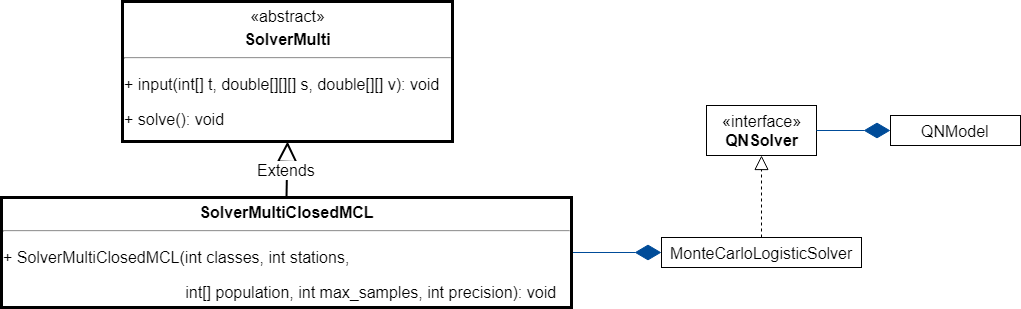
\includegraphics[width=1.\textwidth]{figures/DevGuideUML.png}
\caption{ UML for SolverMulti Interface}
\label{fig:DevGuideUML}
\end{figure}

The Logistic Sampling algorithm is available for use through the \texttt{SolverMultiClosedMCL} class which implements the abstract class \texttt{SolverMulti}. This relationship is summarized in figure \ref{fig:DevGuideUML} The steps to use are as follows:

\begin{itemize}[noitemsep]
    \item Instantiate a \texttt{SolverMultiClosedMCL} object by calling its constructor: \texttt{SolverMultiClosedMCL(int classes, int stations, int[] population, int max\_samples, int precision)}
    \item Call \texttt{input(int[] t, double[][][]s, double[][] v)} to specify the model
    \item Call \texttt{solve()} to calculate the various performance metrics.
    \item The performance metrics are available throught the various getter methods declared in \texttt{SolverMulti}.
\end{itemize}

The constructor, \texttt{input()}, and \texttt{solve()} methods are described in table \ref{table:descriptions_of_methods}.

\begin{table}[H]
\centering
\begin{tabularx}{\textwidth}{@{}lXX@{}}
\toprule
Method  & Description \\ \midrule
Constructor   & Number of \texttt{classes} and \texttt{stations} are specified as \texttt{ints}, and \texttt{population} is specified as an array of \texttt{ints}. Number of samples to integrate over is specified in the fourth argument \texttt{max\_samples}. \texttt{precision} is the number of (base 10) digits that are used in the \texttt{BigDecimal} operations within the solver.\\\\
\texttt{input} & To specify the model, the types of the model are specified through an array of ints: \texttt{int[] t}. These can be \texttt{0} (LD), \texttt{1} (LI), and \texttt{2} (DELAY). For \texttt{LD} models, only multiserver types are supported. \newline \newline
For service times, this is represented through the second argument \texttt{double[][][] s}, where the first two dimensions of this 3-dimensional array is of length \texttt{classes} and \texttt{stations}. For \texttt{LI} and \text{DELAY} stations, the 3rd dimension is of length 1, for \texttt{LD} stations, the 3rd dimension is of length \texttt{population[r]} where \texttt{r} is the class referred to by that entry of the demand matrix. Furthermore, since the solver can only handle multi-server cases, the format of \texttt{double[][][] s} must be the following: 
\begin{equation*}
    \texttt{s[k][r][n]} = s_{kr} * \min(m,n)
\end{equation*}
Where \(s_{kr}\) is the service time associated with a single server in that station, and \(m\) is the number of servers of the station, and \(n\) is the class population considered. The above input must be correct up to 3 decimal places, and the solver will attempt to infer the value of  \(s_{kr}\) and \(m\), and print the server count on the screen.
\\\\
\texttt{solve()}  & When called, instantiates a \texttt{MonteCarloLogisticSolver} which will calculate the stationary point and its hessian of the logistic integrand. Then it will perform Monte Carlo integration over the specified logistic function, and store the values of the performance metrics. \\ \bottomrule
\end{tabularx}
\caption{Descriptions of methods}
\label{table:descriptions_of_methods}
\end{table}

\newpage

\section{Short guide for GUI users}

To use the Logistic Sampling Algorithm, selected \texttt{Logistic Sampling} from the drop down menu:
\begin{figure}[H]
\centering
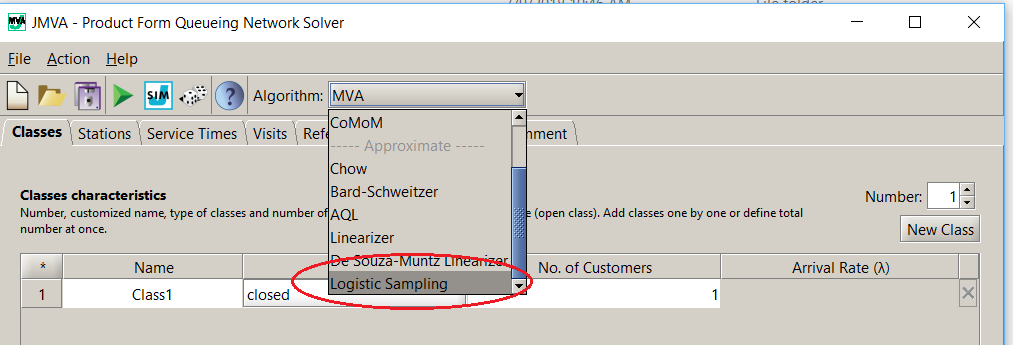
\includegraphics[width=1.\textwidth]{figures/LogisticSampling_GUI_selection.png}
\caption{ Solver Selection Menu }
\label{fig:LogisticSampling_GUI_selection}
\end{figure}

The Logistic Sampling Solver hypter-parameters have to be specified. \texttt{Max Samples} represent the number of samples for which the Monte Carlo Integration will be carried out with. \texttt{Precision} represents the number of (base 10) digits which the \texttt{BigDecimal} operations will use in the algorithm.

\begin{figure}[H]
\centering
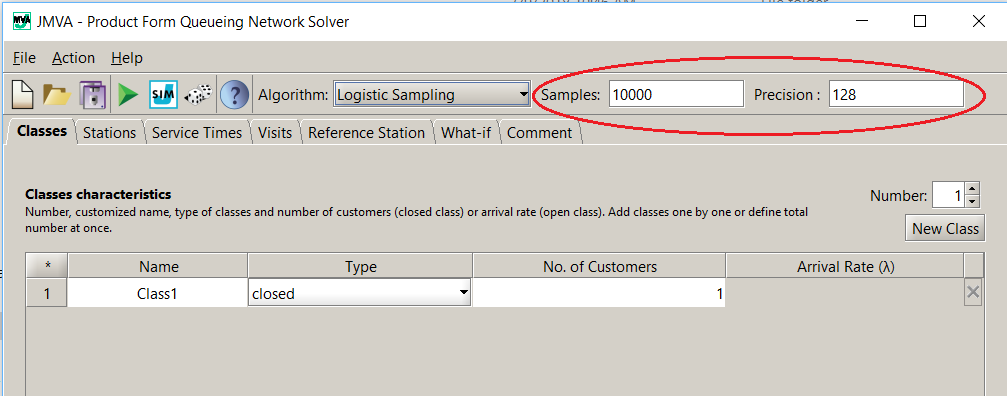
\includegraphics[width=1.\textwidth]{figures/LogisticSampling_GUI_hyperparams.png}
\caption{ Solver hyper-parameter specification }
\label{fig:LogisticSampling_GUI_hyperparams}
\end{figure}

To specify service times, one can enter a single number for \texttt{Load Independent} or \texttt{Delay} servers. For \texttt{Load Dependent} servers, the entries must be of the format:
\begin{equation*}
    \texttt{s[k][r][n]} = s_{kr} * \min(m,n)
\end{equation*}
Where \texttt{s[k][r][n} is the load-dependent service time for station \(k\), class \(r\), and for population \texttt{n}. \(s_{kr}\) is the service time associated with a single server in that station. \(m\) is the number of servers in that station. This number must be specified correctly to 3 decimal places. The solver will then attempt to infer the values of \(m\) and \(s_{kr}\) and display it to the console as confirmation.
\\\\
Shown below is the service time inputs for \textit{single-class 3-station model} with the following definitions for the 3 stations. Population for class 0 is \(4\):
\begin{itemize}[noitemsep]
    \item \textbf{Station 0}: Load independent with service time \(s_{00} = 2\)
    \item \textbf{Station 1}: Delay with service time \(s_{10} = 3\)
    \item \textbf{Station 2}: Multiserver with service time \(s_{20} = 8\) and \(m = 3\).
\end{itemize}

\begin{figure}[H]
\centering
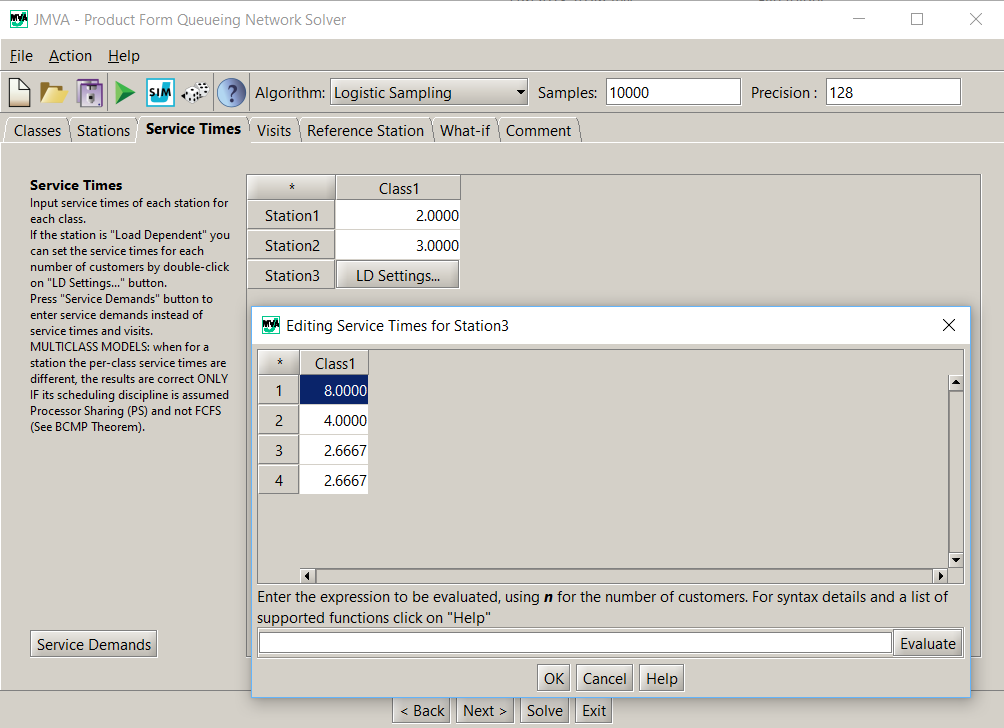
\includegraphics[width=1.\textwidth]{figures/LogisticSampling_GUI_input.png}
\caption{ Solver input }
\label{fig:LogisticSampling_GUI_input}
\end{figure}

\newpage

\chapter{LSEPI Ethics Checklist}
\section{Discussion of Ethics in the Project}

The option 'yes' was checked for the following points in section 8 of the checklist (dual use):
\begin{itemize}
    \item Does your project have the potential for military applications?
    \item Does your project have an exclusive civilian application focus?
\end{itemize}

The aim of this project was for the research and optimization of civilian computer systems. However, it is possible that such tools can be used in a military context. Analytical modelling of computer systems, which is the primary function of software developed in this project, has a purely constructive role: to be able to model and predict performance of complex computer systems. However, it is also possible that such modelling tools be used as weapons to aid coordinated cyber-attacks. Being able to model and predict computer systems accurately , may be used in a military context to target vulnerable systems. However, this requires intimate knowledge of the system that is targeted, and it has never been used in such a context.
\\\\
In conclusion, while there may be a possibility of military use for the research software tools developed in this project, it is extremely unlikely that it would be used. There are no other major ethical concerns besides the one outlined above.

\newpage

\section{LSEPI Ethics Checklist}

\begin{figure}[H]
\begin{center}
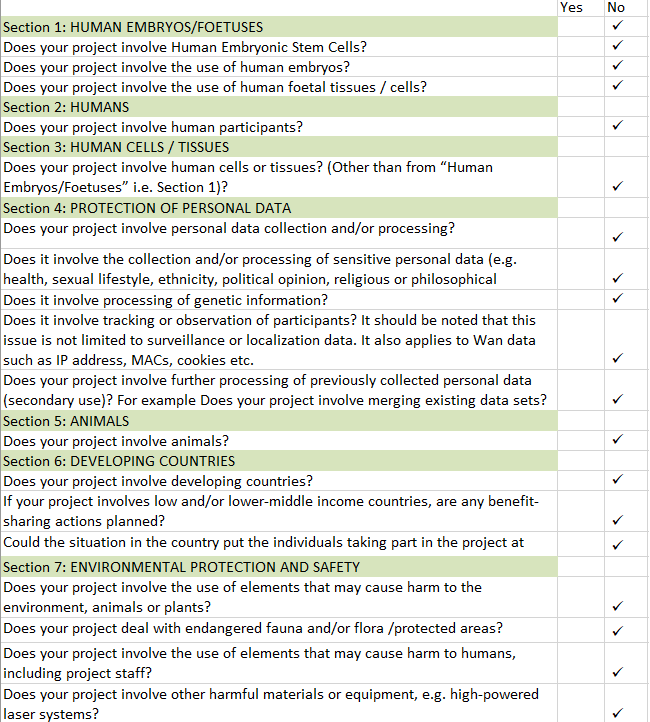
\includegraphics[width=\textwidth]{Chapter8_Ethics/ethhics_p1.png}
\label{fig:ethics_p1}
\end{center}
\end{figure}

\newpage

\begin{figure}[H]
\begin{center}
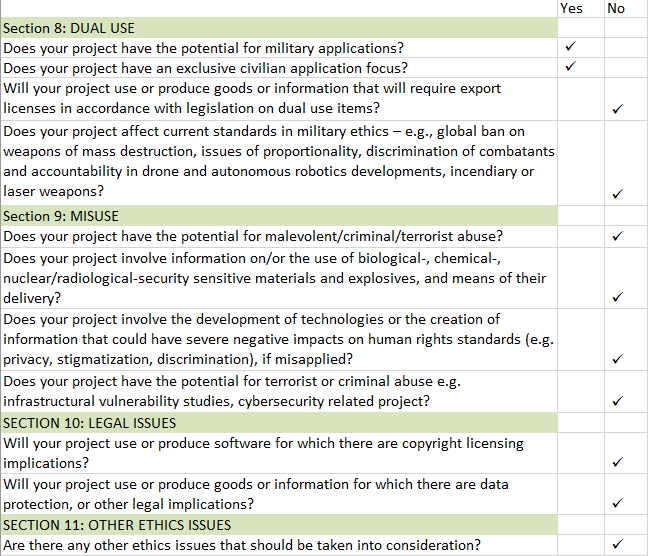
\includegraphics[width=\textwidth]{Chapter8_Ethics/ethhics_p2.png}
\label{fig:ethics_p2}
\end{center}
\end{figure}